\documentclass[11pt, oneside]{article} 
\usepackage{geometry}
\geometry{letterpaper} 
\usepackage{graphicx}
	
\usepackage{amssymb}
\usepackage{amsmath}
\usepackage{parskip}
\usepackage{color}
\usepackage{hyperref}

\graphicspath{{/Users/telliott_admin/Tex/png/}}
% \begin{center} 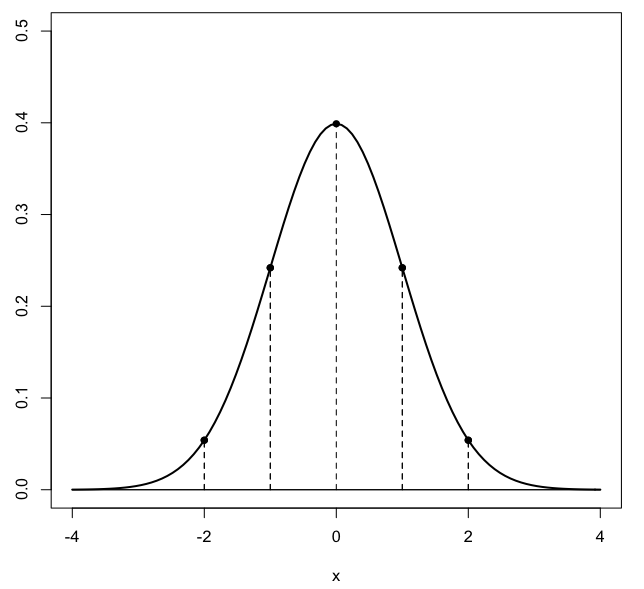
\includegraphics [scale=0.4] {gauss3.png} \end{center}

\title{Elliptic curve cryptography}
\date{}

\begin{document}
\maketitle
\Large
This is a brief overview of the properties of elliptic curves over discrete finite fields such as the integers with a modulus, which are employed in public key cryptosystems.

Most of the material is taken from this source:

\url{https://www.youtube.com/watch?v=F3zzNa42-tQ}

Elliptic curves consist of the points that satisfy an equation of the form
\[ y^2 = x^3 + ax + b \]
for some $a,b,x,y$ taken from a particular field, e.g. the real numbers, or even a discrete finite field (like a subset of the integers).

Elliptic equations can be connected to a problem we know.  The sum of squares of the first $x$ integers is

\begin{center} 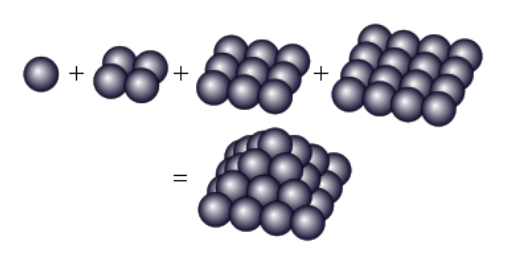
\includegraphics [scale=0.4] {sum_sq.png} \end{center}
\[ \frac{x(x + 1)}{2} \ \frac{2x + 1}{3} \]
We ask for solutions where this expression is equal to a perfect square.
\[ y^2 = \frac{x(x + 1)}{2} \ \frac{2x + 1}{3} = \frac{1}{6} \ [ \ 2x^3 + 3x^2 + 1 \ ] \]

Obviously, this is not quite the elliptic form.

But it turns out that the quadratic term can be removed from a cubic
\[ z^3 + mz^2 + nz + o \]
by an inspired substitution, $z = x - m/3$.  We don't have to figure this whole thing out, just track the quadratic terms. With the substitution
\[ (x-\frac{m}{3})^3 + m(x-\frac{m}{3})^2 + \dots \]

Expansion of the second term gives one quadratic, $mx^2$.

The cubic binomial has cofactors of $3$ for the inner terms so the first term gives
\[ (x-\frac{m}{3})^3 = x^3 + 3x^2(-\frac{m}{3}) + \dots \]

This part has one quadratic $-mx^2$, which just cancels the other factor of $mx^2$. The result (lacking a quadratic term), is called a depressed cubic.  The factor of $1/3$ in the substitution just cancels the factor of $3$ from the binomial.

\url{}

Elliptic equations don't have much to do with actual ellipses, whose formulas are quadratic.  It is said that such equations arise in integrals to determine the arc length of an ellipse, but I haven't made the connection yet to the formulation of this integral that I know.

\subsection*{example}
With $a=-1, b = 2$ we have
\[ y^2 = x^3 - x + 2 \]
\[ y = \sqrt{x^3 - x + 2} \]
Here is a plot of the positive root.

\begin{center} 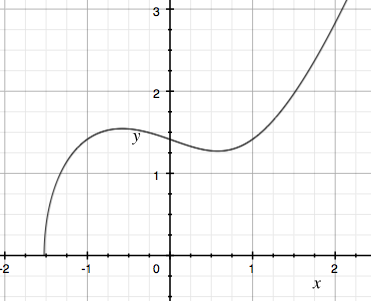
\includegraphics [scale=0.6] {elliptic.png} \end{center}

Normally, we include both the positive and negative roots, and the result (for some values of $a$ and $b$) is a knob-shaped structure.  You can see more examples at

\url{https://en.wikipedia.org/wiki/Elliptic_curve}

A restriction on the values $a$ and $b$ is that $4a^3 + 27b^2 \ne 0$.  The reason for this is that these values yield curves with cusps where the curve collapses (coalesces into a point) or crosses over itself.

Elliptic curves may be defined over different fields, such as $\mathbb{R}$, $\mathbb{Q}$, $\mathbb{C}$, or even values drawn from a subset of the integers, as we will use here.

A field is a set on which addition and multiplication are defined.  The addition operation is not necessarily defined in the same way as the elementary one.

Additionally, for this application the set must include the "point at infinity".  This is given in the video as 
\begin{center} 
\includegraphics [scale=0.5] {infinity_point.png} \end{center}
However, I haven't found a way to typeset it yet, so I will just spell it out when we need it.

Let's start by looking at one elliptic curve over $\mathbb{R}$:
\[ y^2 = x^3 + 2x + 2 \]

Addition can be defined graphically by drawing  a line through two points $P$ and $Q$

\begin{center} 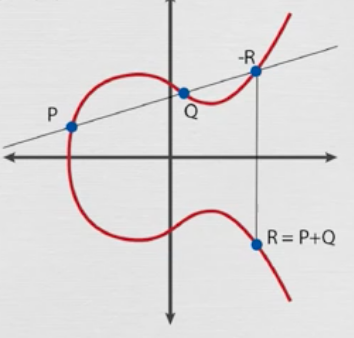
\includegraphics [scale=0.5] {elliptic_addition.png} \end{center}
The third intersection with the elliptic curve, when reflected across the $x$-axis, is the resulting point $R$.
\[ P + Q = R \]

Notice that the reflection of $-R$ is $R$.  Addition of $R + (-R) =$ "the point at infinity".

The special case where $P = Q$ is called point doubling.  Draw the tangent to the curve at $P$ and find its intersection with the curve.

\begin{center} 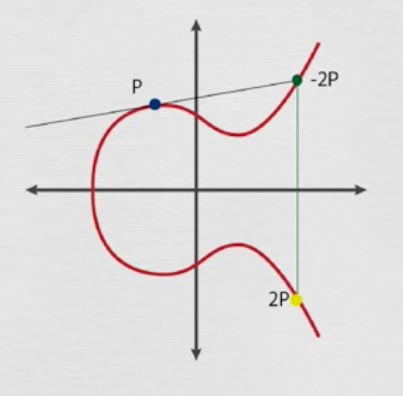
\includegraphics [scale=0.5] {elliptic_doubling.png} \end{center}
This is just like the definition of differentiation in calculus.  Instead of the line from $P$ to $Q$ seen when adding $P + Q$, as $Q$ approaches $P$ we get the tangent.

Multiplication is simply defined to be repeated addition, which is the same as the elementary operation.  For example
\[ 5 \times P = P + P + P + P + P \]

\subsection*{finite field with integers}
Cryptography uses subsets of the field of positive and negative integers (plus zero) mod some largest value, $p$.  The field is denoted as $\mathbb{Z}/p \mathbb{Z}$.  The notation uses $\mathbb{Z}$ (the set of positive and negative integers plus zero), because some intermediate calculations involve negative integers.  However, the points (ordered pairs of values) in the final field have components $\ge 0$.

All of the arithmetic is done with $p$ as the modulus, so at any stage one can take the remainder from division by $p$ without changing the result.  Any value which is less than $0$ is computed by adding $p$ to it until it becomes greater than or equal to zero.

Here is the example we develop below, where the modulus is $17$.  (This is just a tractable example.  For actual cryptography there might be something like 50 digits in  $a$ and $b$ in decimal format and usually more like 256 bits worth of information.)

Points shown in blue comprise the field, a subset of $\mathbb{Z}/17 \mathbb{Z}$.
\begin{center} 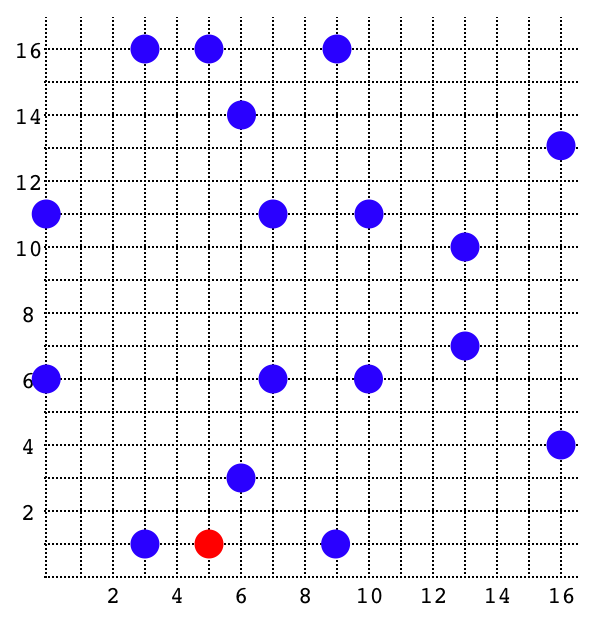
\includegraphics [scale=0.4] {elliptic_mod2.png} \end{center}

The points we will generate are ordered pairs $(x,y)$, where $0 \le x < p$ and $0 < y < p$.  

Less than 10\% of all points on the grid are in the field.  There are $289$  locations on the grid and only $18$ points in the field.  The shape is reminiscent of
\[ y^2 = x^3 + ax + b \]

\emph{All points shown are solutions} to this equation, even if it is not apparent at first.  This is a result of the modular arithmetic. 

$(5,1)$ is clearly a solution.  It is the point marked in red.  
\[ 5^3 + 2 \times 5 + 2 = 137 \ \text{ mod } 17 = 1 \]
$(5,16)$ is also a solution.  That's because $16^2 = 256$ mod $17 = 1$.

More systematically, let's write a Python script to compute $y^2$ from the equation.  The $x$ values are in the first line of output and the corresponding $y^2$ values are in the second.
\begin{verbatim}
 0  1  2  3  4  5  6  7  8  9 10 11 12 13 14 15 16
 2  5 14  1  6  1  9  2  3  1  2 12  3 15  3  7 16
\end{verbatim}
We obtain $(0,6)$ as a solution because $6^2 = 36$ mod $17 = 2$, which matches the value output by the script corresponding to $x = 0$.

Here are the squares of the integers in our field (mod 17).  The $y$ values are in the first line of output, and the corresponding $y^2$ values are in the second.
\begin{verbatim}
 0  1  2  3  4  5  6  7  8  9 10 11 12 13 14 15 16
 0  1  4  9 16  8  2 15 13 13 15  2  8 16  9  4  1
\end{verbatim}

There is no point on the grid corresponding to $x = 1$. That's because the value of $y^2$ from the elliptic equation is $5$ (first script), and there is no integer which squares to give $5$ mod $17$ (second script), so there is no candidate for the point $(1,y)$.  The same is true for $x=2$.  

However $x = 7$ gives $2$ in the first script, and there are two $y$ values that give $y^2 = 2$ (mod 17).  Thus, $(7,6)$ and $(7,11)$ are in our field.

\subsection*{algebraic rules}
The graphical methods for addition and doubling are apparently not valid for this modular example, although addition seems to work in one case (not shown).

We proceed by using the algebraic formulas given in the video (and other sources).  All computation from this point will use these rules.  We will derive them after working through examples for point addition ($P + Q$) and point doubling ($P + P$).

For carrying out the addition operation on two points $P$ and $Q$ (finding $P + Q$), first the slope $s$ of the line joining $P$ and $Q$ is defined in the usual way to be
\begin{equation}
s = \frac{\Delta y}{\Delta x} = \frac{y_Q - y_P}{x_Q - x_P}
\end{equation}

The new point $x_R$ is computed as follows:
\begin{equation}
x_R = s^2 - (x_P + x_Q)
\end{equation}

That slope $s$ is also the slope of the line joining $P$ and $-R$ (minus, because the point is reflected across the $x$-axis) so
\[ s = \frac{y_{-R} - y_P}{x_R - x_P} = \frac{-y_R - y_P}{x_R - x_P} = \frac{y_R + y_P}{x_P - x_R} \]
and it follows that 
\begin{equation}
y_R = s(x_P - x_R) - y_P
\end{equation}

For point doubling with the point $P$ (finding $P + P$), the slope is computed as:
\begin{equation}
s = \frac{3x_P^2 + a}{2y_P}
\end{equation}

The equations to find the new $x$ and $y$ are the same for both methods.

In the special case where $x_P = x_Q$ and the graphical line is vertical, then the result of addition is the "point at infinity".  The same is true for point doubling if $x_P = 0$ (extreme left-hand point of the curve).

\subsection*{derivations}

Equation (4) can be derived by implicit differentiation of the elliptic curve equation:
\[ y^2 = x^3 + ax + b \]
\[ 2y \ dy = (3x^2 + a) \ dx \]
\[ s = \frac{dy}{dx} = \frac{3x^2 + a}{2y} \]
Now just substitute $x = x_P, y = y_P$.

Equation (2) is plausible considering that if we have the system
\[ x^3 + ax + b \]
and the line $y = \alpha x + \beta$
\[ (\alpha x + \beta)^2 = x^3 + ax + b \]

This is a cubic, thus there are three roots.  According to Kak

\url{https://engineering.purdue.edu/kak/compsec/}

(Lecture 14), a standard result is that the three roots added together equal $\alpha^2$:
\[ x_P + x_Q + x_R = \alpha^2 \]
or $s^2$ using the previous notation.

I found a proof of the last result here:

\url{http://wstein.org/simuw06/ch6.pdf}

The line through $P$ and $Q$ (and $-R$) is
\[ y = y_P + s(x - x_P) \]
Substituting into
\[ y^2 = x^3 + ax + b \]
\[ (y_P + s(x - x_P))^2 = x^3 + ax + b \]
We don't have to multiply this out.  The low-order terms (constant and constant times $x$) won't be needed.  

If we ignore those, we will have $sx^2$ from the left-hand side and $x^3$ from the right, so gathering everything on one side, we obtain 
\[ f(x) = x^3 - s^2 x^2 + \dots = 0 \]

Now, we know that $x_P$ and $x_Q$ are roots of $f$.  For the elliptic curves we use, there are three distinct roots.  So write
\[ f(x) = 0 = (x - x_P)(x - x_Q)(x - x_R) \]
Equating the two expressions, we have
 \[ x^3 - s^2 x^2 + \dots = 0 = (x - x_P)(x - x_Q)(x - x_R) \]
If we multiply out the right-hand side, the coefficient of $x^2$ will be $(-x_P - x_Q - x_R)$ and so
\[ -s^2 = -x_P - x_Q - x_R \]
\[ s^2 = x_P + x_Q + x_R \]
\[ x_R = s^2 - (x_P + x_Q) \]
This is equation (2).

$\square$

\subsection*{generator}
Our example is the field with 17 as the modulus and the particular elliptic curve is
\[ y^2 = x^3 + 2x + 2 \ \text{ (mod } 17) \]

A convenient way is to obtain all the points in the field is to use a \emph{generator}.  We pick a base point, an ordered pair $(x,y)$ that solves the equation.  Suppose we pick $G = (5,1)$.  

Re-check that $x$ and $y$ do satisfy the equation:
\[ 5^3 + 2 \times 5 + 2 = 137  \ \text{ (mod } 17) = 1 = y^2 \]

Use the slope equation for point doubling:
\[ s = \frac{3 \times x_P^2 + a}{2 \times y_P} \]
\[ = \frac{3 \times 5^2 + 2}{2 \times 1} \]
\[ = \frac{77}{2} = 77 \times 2^{-1}  \]

We haven't talked about division before.  Division is accomplished in modular arithmetics by using the multiplicative inverse (MI).  For this example, we need the MI of $2$ (mod 17).  For the general solution to this problem, use the Extended Euclidean Algorithm.  I've written about this extensively, so I won't repeat that here.

In this very simple group, we find that since $2 \times 9 = 18$ (mod 17) $ = 1$, the MI of $2$ is $9$.  

Thus
\[ s = 77 \times 9 = 693   \ \text{ (mod } 17) = 13 \]
And then
\[ x_R = s^2 - (x_P + x_Q) \]
\[ = 13^2 - (5 + 5) = 159 \ \text{ (mod } 17) = 6  \] 
We obtain $y$ by using the equation we had above
\[ y_R = s(x_P - x_R) - y_P \]
\[ = 13 (5 - 6) - 1 = -14 \ \text{ (mod } 17) = 3  \] 
Here we have used the fact that a number less than 0 mod n is computed by adding enough copies of $p$ to it until it is $\ge 0$.

We can also plug in
\[ y^2 = x^3 + 2x + 2 \ \text{ (mod } 17) \]
\[ = 6^3 + 12 + 2 = 230   \ \text{ (mod } 17) = 9 \]
So $y = 3$ and $2G = (6,3)$.

\subsection*{extension}

We compute the other powers of $2$ ($4G, 8G$, etc.) by point doubling.

The rest of the values are computed by addition.  For example
\[ 3G = G + 2G = (5,1) + (6,3) \]
with
\[ s = \frac{y_Q - y_P}{x_Q - x_P} = \frac{2}{1} = 2 \]
so
\[ x_R = s^2 - (x_P + x_Q) \]
\[ = 2^2 - (11) = -7  \ \text{ (mod } 17)  = 10 \]
and
\[ y_R = s(x_P - x_R) - y_P \]
\[ = 2(-5) - 1 = -11 = 6 \]
We have that $3G = (10,6)$.

It is interesting and reassuring that, for example:
\[ 6G = 5G + G = 4G + 2G \]
and it is also equal to $3G$ doubled.  [ Verify this ]

We continue until finally $18G = (5,16)$.  Since $18G$ is the same $x$ as for $G$, the slope calculated for $19G = 18G + G$ is infinite, and the result is equal to "the point at infinity".

Notice that the number of points in the field $n$ is $18$, which is larger than $p$.

At the very end of this write-up is a Python script (\textbf{eutils.py}) that contains functions to implement the algebra.  We can use it to calculates all the points up to $18G$, with any starting point.  To begin with, we choose to start with $(5,1)$.

The points are output in palindromic form:  the $x$ values form the series:
\begin{verbatim}
 5  6 10  3  9 16  0 13  7  7 13  0 16  9  3 10  6  5 
\end{verbatim}

Since the last point has $x=5$, as does the first, the next point will be "the point at infinity."

The index, $x$ and $y$ values are

\begin{verbatim}
 1  2  3  4  5  6  7  8  9 10 11 12 13 14 15 16 17 18
 5  6 10  3  9 16  0 13  7  7 13  0 16  9  3 10  6  5
 1  3  6  1 16 13  6  7  6 11 10 11  4  1 16 11 14 16
\end{verbatim}

It is worth noting that any of the points on the elliptic curve for this example can be chosen as a generator.  All the same points will be generated, but the order will be different.  Here is output for points with index 2-5 above:

\begin{verbatim}
 > python script.py 6 3
 1  2  3  4  5  6  7  8  9 10 11 12 13 14 15 16 17 18
 6  3 16 13  7  0  9 10  5  5 10  9  0  7 13 16  3  6
 3  1 13  7 11 11  1 11 16  1  6 16  6  6 10  4 16 14
> python script.py 10 6
 1  2  3  4  5  6  7  8  9 10 11 12 13 14 15 16 17 18
10 16  7  0  3  5  6  9 13 13  9  6  5  3  0  7 16 10
 6 13  6 11 16 16  3 16  7 10  1 14  1  1  6 11  4 11
> python script.py 3 1
 1  2  3  4  5  6  7  8  9 10 11 12 13 14 15 16 17 18
 3 13  0 10  5  9  7 16  6  6 16  7  9  5 10  0 13  3
 1  7 11 11  1 16  6  4 14  3 13 11  1 16  6  6 10 16
> python script.py 9 16
 1  2  3  4  5  6  7  8  9 10 11 12 13 14 15 16 17 18
 9  7  3  5 16 13 10  6  0  0  6 10 13 16  5  3  7  9
16 11 16  1 13 10 11  3  6 11 14  6  7  4 16  1  6  1
>\end{verbatim}

You can see what the pattern is.  Starting with the second point yields all the points with an even index in the original output, followed by all the points with an odd index.  Starting with the third point yields every third point, etc.

This dependence means that, in addition to the curve parameters $a$ and $b$ and the modulus $p$, we also need to specify the base point or generator $G$, which is an ordered pair.

Can we go beyond $G18$?  In principle we can.
\[ G2 + G18 = (6,3) + (5,16) \]
\[ s = \frac{13}{-1} = \frac{13}{16} = 13 \times 16^{-1} \]
\[ = 13 \times 16 = 208 \text{ mod } 17 = 4  \]

\[ x_R = s^2 - (x_P + x_Q) \]
\[ = 16 - (11) = 5 \]

\[ y_R = s(x_P - x_R) - y_P \]
\[ = 4 \times (1) - 3 = 1 \]
The new point is $G20 = (5,1)$.  We're back where we started.

In practice, we never do this, because we will pick numbers $\alpha$ and $\beta$ both $ < n$.

\subsection*{one-way or trapdoor functions}
For the RSA method, the security of the algorithm depends on the fact that it is simple to multiply two large primes $p$ and $q$ together to form their product $p \times q = n$, but infeasible to start with $n$ and find its prime factors.

Elliptic curves over finite fields have a similar one-way property, namely that if we pick an integer $1 \le k \le n$, it is not too hard to compute the multiple of the generator point in the field $kG = Q$, but it is infeasible to find the value of $k$, knowing $Q$.

This is called the \textbf{discrete logarithm problem}.

The result is actually a bit surprising.  If we were to add the generator point to itself $k$ times, as described above, this would be the same amount of work as an attacker would have to do using brute force to guess $k$, knowing $Q$.

Nevertheless, the basic idea is then that Alice chooses a secret key $\alpha$ and computes and broadcasts $A$ over the insecure channel to Bob.  Bob does the same with $\beta$ and broadcasts $B$.

Even knowing $A$ and $B$ (and $G$ and $n$), an eves-dropper Eve cannot find $\alpha$ or $\beta$ but Alice and Bob can both easily compute:

\[ P = \alpha B = \beta A = \alpha \ \beta G \]
and they can use this information to derive a secret key or do other things that can be accomplished with asymmetric cryptography.

\subsection*{calculation}

Below is a Python script that calculates all the points, as shown

\begin{verbatim}
a = 2
b = 2
n = 17

# multiplicative inverses mod n = 17
D = {1:1, 2:9, 3:6, 4:13, 5:7, 
     8:15, 10:12, 11:14, 16:16}   
for k,v in D.items():  D[v] = k

# square roots
sqrtD = {1:(1,16), 2:(6,11), 4:(2,15), 
     8:(5,12), 9:(3,14), 
     13:(8,9), 15:(7,10), 16:(4,13)}   

def check(x,y):
  def f(x):
    return (x**3 + a*x + b) % n
  y_sq = f(x)
  ysqrts = sqrtD[y_sq]
  assert y in ysqrts
  #print x, y, ysqrts

def getx(s, x1, x2):
  return (s**2 - (x1 + x2)) % n

def gety(s,(x,y),X):
  return (s*(x-X) - y)  % n

def add((x,y),(x2,y2)):
  num = (y2 - y)
  den = (x2 - x) % n
  s = (num * D[den]) % n
  X = getx(s,x,x2)
  return X, gety(s,(x,y),X)

def double((x,y), a=a):
  num = (3 * x**2 + a)
  den = (2 * y) % n
  s = (num * D[den]) % n
  X = getx(s,x,x)
  return X, gety(s,(x,y),X)

def makeG((x,y)):
  # 1G
  G = { 1:(x,y) }
  check(x,y)
  
  # 2G, 4G, 8G, 16G
  for i in range(4):
    X,Y = double((x,y))
    k = 2**(i+1)
    G[k] = (X,Y)
    x,y = X,Y
    check(x,y)
    
  # 3G..18G
  x,y = G[2]
  for i in range(3,19):
    X,Y = add(G[1],(x,y))
    if not i in G:
      G[i] = (X,Y)
    else:
      assert G[i] == (X,Y)
    x,y = X,Y
    check(x,y)
  return G
\end{verbatim}

The code to exercise this is in \textbf{script.py}

\begin{verbatim}
import sys
from eutils import *

x,y = 5,1
if len(sys.argv) > 1:
  x = int(sys.argv[1])
  y = int(sys.argv[2])

G = makeG((x,y))
L = sorted(G.keys())

# fancy printing
for i in L:
  print str(i).rjust(2),
print

for i in L:
  X = G[i][0]
  print str(X).rjust(2),
print

for i in L:
  Y = G[i][1]
  print str(Y).rjust(2),
print
\end{verbatim}

This matches what is in the video.

\end{document}